% Springer SVMult contribution manuscript based on the supplied Springer-Template-latex/author/authorsample.tex.
% The source template uses svmult.cls, graybox, newtxtext/newtxmath, and spmpsci.
\documentclass[graybox]{svmult}

\usepackage{type1cm}
\usepackage{makeidx}
\usepackage{graphicx}
\usepackage{multicol}
\usepackage[bottom]{footmisc}
\usepackage{newtxtext}
\usepackage{newtxmath}
\usepackage{array}
\usepackage{booktabs}
\usepackage{tabularx}
\usepackage{xcolor}
\usepackage{textcomp}
\usepackage{url}
\usepackage{hyperref}
\hypersetup{hidelinks}
\graphicspath{{figures/}}

\makeindex
\let\svbibliography\thebibliography
\let\endsvbibliography\endthebibliography
\renewenvironment{thebibliography}[1]{\svbibliography{#1}\scriptsize}{\endsvbibliography}

\begin{document}

% Generated from artifacts/raw CSV outputs; do not hand edit.
\newcommand{\FEVERDensePrecision}{0.849}
\newcommand{\FEVERDenseRecall}{1.000}
\newcommand{\FEVERDenseFOne}{0.896}
\newcommand{\FEVERDenseRephrase}{1.000}
\newcommand{\FEVERDenseComposable}{0.659}
\newcommand{\FEVERDenseSourceFOne}{0.152}
\newcommand{\FEVERLexicalPrecision}{0.987}
\newcommand{\FEVERLexicalRecall}{1.000}
\newcommand{\FEVERLexicalFOne}{0.992}
\newcommand{\FEVERLexicalRephrase}{1.000}
\newcommand{\FEVERLexicalComposable}{0.660}
\newcommand{\FEVERLexicalSourceFOne}{0.152}
\newcommand{\FEVERXProvPrecision}{0.879}
\newcommand{\FEVERXProvRecall}{1.000}
\newcommand{\FEVERXProvFOne}{0.917}
\newcommand{\FEVERXProvRephrase}{1.000}
\newcommand{\FEVERXProvComposable}{0.660}
\newcommand{\FEVERXProvSourceFOne}{0.152}
\newcommand{\FEVERN}{19998}
\newcommand{\SciFactDensePrecision}{0.312}
\newcommand{\SciFactDenseRecall}{1.000}
\newcommand{\SciFactDenseFOne}{0.421}
\newcommand{\SciFactDenseRephrase}{1.000}
\newcommand{\SciFactDenseComposable}{0.563}
\newcommand{\SciFactDenseSourceFOne}{0.132}
\newcommand{\SciFactLexicalPrecision}{0.994}
\newcommand{\SciFactLexicalRecall}{1.000}
\newcommand{\SciFactLexicalFOne}{0.996}
\newcommand{\SciFactLexicalRephrase}{1.000}
\newcommand{\SciFactLexicalComposable}{0.563}
\newcommand{\SciFactLexicalSourceFOne}{0.132}
\newcommand{\SciFactXProvPrecision}{0.445}
\newcommand{\SciFactXProvRecall}{1.000}
\newcommand{\SciFactXProvFOne}{0.552}
\newcommand{\SciFactXProvRephrase}{1.000}
\newcommand{\SciFactXProvComposable}{0.563}
\newcommand{\SciFactXProvSourceFOne}{0.132}
\newcommand{\SciFactN}{300}
\newcommand{\PubHealthDensePrecision}{0.206}
\newcommand{\PubHealthDenseRecall}{1.000}
\newcommand{\PubHealthDenseFOne}{0.302}
\newcommand{\PubHealthDenseRephrase}{1.000}
\newcommand{\PubHealthDenseComposable}{0.856}
\newcommand{\PubHealthDenseSourceFOne}{0.183}
\newcommand{\PubHealthLexicalPrecision}{0.923}
\newcommand{\PubHealthLexicalRecall}{0.932}
\newcommand{\PubHealthLexicalFOne}{0.909}
\newcommand{\PubHealthLexicalRephrase}{0.932}
\newcommand{\PubHealthLexicalComposable}{0.777}
\newcommand{\PubHealthLexicalSourceFOne}{0.183}
\newcommand{\PubHealthXProvPrecision}{0.333}
\newcommand{\PubHealthXProvRecall}{1.000}
\newcommand{\PubHealthXProvFOne}{0.437}
\newcommand{\PubHealthXProvRephrase}{1.000}
\newcommand{\PubHealthXProvComposable}{0.856}
\newcommand{\PubHealthXProvSourceFOne}{0.183}
\newcommand{\PubHealthN}{1220}
\newcommand{\PubHealthEvidenceDensePrecision}{0.158}
\newcommand{\PubHealthEvidenceDenseRecall}{1.000}
\newcommand{\PubHealthEvidenceDenseFOne}{0.258}
\newcommand{\PubHealthEvidenceDenseRephrase}{1.000}
\newcommand{\PubHealthEvidenceDenseComposable}{0.727}
\newcommand{\PubHealthEvidenceDenseSourceFOne}{0.205}
\newcommand{\PubHealthEvidenceLexicalPrecision}{0.737}
\newcommand{\PubHealthEvidenceLexicalRecall}{0.916}
\newcommand{\PubHealthEvidenceLexicalFOne}{0.779}
\newcommand{\PubHealthEvidenceLexicalRephrase}{0.916}
\newcommand{\PubHealthEvidenceLexicalComposable}{0.605}
\newcommand{\PubHealthEvidenceLexicalSourceFOne}{0.205}
\newcommand{\PubHealthEvidenceXProvPrecision}{0.266}
\newcommand{\PubHealthEvidenceXProvRecall}{1.000}
\newcommand{\PubHealthEvidenceXProvFOne}{0.389}
\newcommand{\PubHealthEvidenceXProvRephrase}{1.000}
\newcommand{\PubHealthEvidenceXProvComposable}{0.727}
\newcommand{\PubHealthEvidenceXProvSourceFOne}{0.205}
\newcommand{\PubHealthEvidenceN}{33}
\newcommand{\FEVERDenseFOneCI}{0.896 [0.894, 0.899]}
\newcommand{\FEVERLexicalFOneCI}{0.992 [0.991, 0.992]}
\newcommand{\FEVERXProvFOneCI}{0.917 [0.915, 0.919]}
\newcommand{\SciFactDenseFOneCI}{0.421 [0.390, 0.452]}
\newcommand{\SciFactLexicalFOneCI}{0.996 [0.992, 0.999]}
\newcommand{\SciFactXProvFOneCI}{0.552 [0.518, 0.585]}
\newcommand{\PubHealthDenseFOneCI}{0.302 [0.290, 0.315]}
\newcommand{\PubHealthLexicalFOneCI}{0.909 [0.901, 0.918]}
\newcommand{\PubHealthXProvFOneCI}{0.437 [0.420, 0.453]}
\newcommand{\PubHealthEvidenceDenseFOneCI}{0.258 [0.209, 0.310]}
\newcommand{\PubHealthEvidenceLexicalFOneCI}{0.779 [0.701, 0.851]}
\newcommand{\PubHealthEvidenceXProvFOneCI}{0.389 [0.318, 0.464]}
\newcommand{\FEVERDensePairFOneDelta}{-0.095 [-0.098, -0.093]}
\newcommand{\FEVERXProvPairFOneDelta}{-0.074 [-0.076, -0.072]}
\newcommand{\FEVERDenseRephraseDelta}{-0.000 [-0.001, -0.000]}
\newcommand{\FEVERXProvRephraseDelta}{0.000 [0.000, 0.000]}
\newcommand{\FEVERDenseComposableDelta}{-0.000 [-0.001, -0.000]}
\newcommand{\FEVERXProvComposableDelta}{0.000 [0.000, 0.000]}
\newcommand{\SciFactDensePairFOneDelta}{-0.575 [-0.603, -0.545]}
\newcommand{\SciFactXProvPairFOneDelta}{-0.444 [-0.477, -0.410]}
\newcommand{\SciFactDenseRephraseDelta}{0.000 [0.000, 0.000]}
\newcommand{\SciFactXProvRephraseDelta}{0.000 [0.000, 0.000]}
\newcommand{\SciFactDenseComposableDelta}{0.000 [0.000, 0.000]}
\newcommand{\SciFactXProvComposableDelta}{0.000 [0.000, 0.000]}
\newcommand{\PubHealthDensePairFOneDelta}{-0.607 [-0.621, -0.593]}
\newcommand{\PubHealthXProvPairFOneDelta}{-0.473 [-0.491, -0.455]}
\newcommand{\PubHealthDenseRephraseDelta}{0.068 [0.061, 0.075]}
\newcommand{\PubHealthXProvRephraseDelta}{0.068 [0.061, 0.075]}
\newcommand{\PubHealthDenseComposableDelta}{0.079 [0.064, 0.094]}
\newcommand{\PubHealthXProvComposableDelta}{0.079 [0.064, 0.095]}
\newcommand{\PubHealthEvidenceDensePairFOneDelta}{-0.522 [-0.600, -0.438]}
\newcommand{\PubHealthEvidenceXProvPairFOneDelta}{-0.391 [-0.480, -0.293]}
\newcommand{\PubHealthEvidenceDenseRephraseDelta}{0.084 [0.039, 0.136]}
\newcommand{\PubHealthEvidenceXProvRephraseDelta}{0.084 [0.041, 0.135]}
\newcommand{\PubHealthEvidenceDenseComposableDelta}{0.122 [0.036, 0.228]}
\newcommand{\PubHealthEvidenceXProvComposableDelta}{0.122 [0.030, 0.229]}
\newcommand{\PAWSTrainLexAUC}{0.496}
\newcommand{\PAWSTrainDenseAUC}{0.634}
\newcommand{\PAWSTrainHybridAUC}{0.554}
\newcommand{\PAWSValidationLexAUC}{0.501}
\newcommand{\PAWSValidationDenseAUC}{0.631}
\newcommand{\PAWSValidationHybridAUC}{0.555}
\newcommand{\PAWSTestLexAUC}{0.495}
\newcommand{\PAWSTestDenseAUC}{0.631}
\newcommand{\PAWSTestHybridAUC}{0.555}
\newcommand{\SciFactSensitivityBest}{0.754}
\newcommand{\SciFactSensitivityPrimary}{0.552}
\newcommand{\SciFactTrainBest}{0.734}
\newcommand{\SciFactTrainBestDense}{0.55}
\newcommand{\SciFactTrainBestHybrid}{0.70}
\newcommand{\FEVERAssertions}{299970}
\newcommand{\SciFactAssertions}{4500}
\newcommand{\PubHealthAssertions}{18315}
\newcommand{\EvidenceAssertions}{495}

\title*{XProv-MAS: Rephrase-Resilient and Composable Semantic Provenance for Cross-Domain Multi-Agent LLM Systems}
\titlerunning{XProv-MAS}
\author{Shivam Sharma}
\authorrunning{Sharma}
\institute{Department of Computer Science and Engineering, Research Manuscript, India \email{research@example.org}}
\maketitle

\abstract{Multi-agent large-language-model systems increasingly produce several textual reports for the same claim, yet their evidence lineage is commonly attached to a surface string, a retrieval rank, or a transient agent identifier. Such representations become brittle when agents rephrase evidence and they do not provide a composable account of which reports describe the same underlying source. This paper presents XProv-MAS, a semantic provenance layer that exposes agent outputs as provenance assertions and links them in a source-oblivious graph using lexical overlap, dense sentence similarity, and a conjunctive semantic gate. The study evaluates the layer on complete or scientifically bounded splits of three established fact-checking resources: 19,998 FEVER development claims, 300 SciFact development claims with 5,183 scientific abstracts, and 1,221 PUBHEALTH development claims, with a separate 33-claim official evidence-document subset. On the fixed primary configuration, XProv-MAS obtains pairwise provenance F1 of \FEVERXProvFOne, \SciFactXProvFOne, \PubHealthXProvFOne, and \PubHealthEvidenceXProvFOne, respectively. Its cross-agent rephrase match is 1.000 on every dataset, while its principal operational advantage is on PUBHEALTH, where it raises composable-source rate from \PubHealthLexicalComposable{} to \PubHealthXProvComposable{} and retains this behavior on the official evidence-document subset. The results also show a boundary condition: lexical linking is more precise on these controlled surfaces, and XProv-MAS does not improve upstream source retrieval. A PAWS audit confirms that dense similarity is more informative than lexical overlap for adversarial paraphrases, but neither scorer solves hard paraphrase matching alone. XProv-MAS is therefore best understood as a provenance-composition layer, not as a replacement for retrieval or fact verification.}
\keywords{Semantic provenance, multi-agent systems, large language models, evidence lineage, fact verification, paraphrase robustness, provenance graphs, reproducibility}

\section{Introduction}

Large language models (LLMs) are increasingly embedded in systems that retrieve evidence, decompose questions, verify claims, summarize documents, and delegate intermediate work to specialized agents. This architecture is useful precisely because agents can search different corpora, use different ranking functions, or produce different explanations. It also creates a provenance problem that is not equivalent to ordinary answer attribution: a final answer may contain several claims, each claim may be supported by several reports, and two reports may refer to one source while using different wording.

The problem is sharpened by rephrasing. Agents commonly normalize, truncate, summarize, or paraphrase evidence before passing it to a verifier, which destroys exact-match identifiers. Conversely, shared title tokens can cause lexical matching to over-compose independent evidence. Provenance systems provide a principled language for entities, activities, agents, and derivations, but their traditional granularity is not sufficient for LLM reports whose semantics are distributed across claims, evidence spans, scores, and transformations. We ask whether a semantic provenance layer can compose independently generated evidence reports without exposing canonical source identifiers to the linker.

This question connects multi-agent coordination, provenance, explainability, retrieval, and semantic robustness. Coordination research treats interaction structure and partial results as first-class objects \cite{Anont4666174668,Anonm202109996w,Anona8023096336,Anonat201801002}; recent LLM-agent work emphasizes workflow and communication but rarely evaluates reusable evidence identity \cite{Anona6024000092,Anona6023067920}. Provenance research connects lineage to accountability and reproducibility \cite{Anonpdinta00119,Anond0182887201,Anonrone0309210,Anonw002cpe6544,Anont15ea000136,Anoni5901717470,Anont2017704893,w3c2013prov}. Explainability and factuality work further shows that plausible text is not a substitute for an inspectable evidence trail \cite{Anone1453561048,Anones201912012,Anonet201807007,Anond6024074210,Anonf602400881z}.

We introduce XProv-MAS, an assertion-level graph that links evidence reports using lexical overlap, dense sentence similarity, and a conjunctive semantic gate. We evaluate it on FEVER, SciFact, and PUBHEALTH, with a separate official PUBHEALTH evidence-document subset, and audit its semantic primitives on PAWS \cite{thorne2018fever,won2020scifact,kotonya2020pubhealth,zhang2019paws}. The contributions are: (i) a source-oblivious assertion representation; (ii) a transparent graph rule for rephrase-aware composition; (iii) a cross-domain evaluation that separates retrieval from linking; and (iv) explicit negative evidence about precision, retrieval ceilings, hard paraphrases, and threshold sensitivity.

\section{Related Work}

Multi-agent systems reconcile partial views produced by agents with different information and objectives. Trust and recommendation studies show that an agent report is not interchangeable with a source-independent fact, while communication surveys emphasize that coordination requires explicit protocols \cite{Anona580079021x,Anonm202109996w,Anona8023096336}. In LLM systems, a planner may ask one agent to retrieve a source, another to challenge it, and a third to summarize both. Each may produce fluent text even when the system cannot determine whether the reports are independent, redundant, or conflicting.

The provenance literature supplies the conceptual foundation for treating evidence as an object with lineage. Workflow systems and scientific-ML studies make activities, inputs, outputs, and transformations inspectable \cite{Anontticsbth361,Anong2010118r86,Anonw002cpe6544}. RO-Crate extends this idea to portable research objects \cite{Anonrone0309210}, and decision provenance connects data flow to accountable systems \cite{Anond0182887201}. XProv-MAS adopts the entity--activity--agent distinction from W3C PROV but applies it to natural-language reports: a controlled rephrase is a derivation, and a graph edge is a tested hypothesis of source identity rather than a supplied identifier.

Lexical overlap is a strong and interpretable similarity baseline but is vulnerable to synonymy, word order, and adversarial substitutions. Sentence embeddings improve semantic sensitivity, although domain shift and hard paraphrases remain difficult \cite{Anona13jair2985,Anonscolia00237,Anonr7901593192,Anonm0219619735,Anona1453593042}. PAWS is useful because its difficult pairs separate word-level overlap from semantic matching \cite{zhang2019paws}. Existing fact-checking and retrieval-augmented-generation studies generally measure label accuracy or evidence relevance; they do not evaluate whether several transformed reports compose into a reusable, source-aware lineage object. This graph-level gap motivates the protocol below.

\section{Methodology}

\subsection{Assertion Representation and Graph Rule}

For query record $r$ and evidence channel $g\in\mathcal{G}$, the system emits an assertion
\begin{equation}
 a_{r,g}=\langle q_r,e_{r,g},g,k_{r,g},s_{r,g},z_{r,g}\rangle,
 \label{eq:assertion}
\end{equation}
where $q_r$ is the claim surface, $e_{r,g}$ is an evidence surface, $k_{r,g}$ is retrieval rank, $s_{r,g}$ is the channel score, and $z_{r,g}$ is a canonical source identifier used only for evaluation. The linker receives the surfaces and channel metadata but not $z_{r,g}$. A report can be rephrased without changing its hidden source, analogous to a PROV derivation \cite{w3c2013prov}.

For surfaces $x$ and $y$, lexical similarity is token Jaccard overlap,
\begin{equation}
 J(x,y)=\frac{|T(x)\cap T(y)|}{|T(x)\cup T(y)|},
 \label{eq:jaccard}
\end{equation}
and dense similarity is cosine similarity between normalized MiniLM sentence embeddings \cite{reimers2020sentence},
\begin{equation}
 D(x,y)=\frac{\phi(x)^{\top}\phi(y)}{\|\phi(x)\|_2\|\phi(y)\|_2}.
 \label{eq:dense}
\end{equation}
We define $H(x,y)=0.35J(x,y)+0.65D(x,y)$. For assertions $i,j$ in one record, XProv-MAS adds an edge when
\begin{equation}
 (H_{ij}\geq\tau_H\;\wedge\;D_{ij}\geq\tau_D)\;\vee\;D_{ij}\geq\tau_{\mathrm{hard}},
 \label{eq:edge}
\end{equation}
with $(\tau_H,\tau_D,\tau_{\mathrm{hard}})=(0.55,0.60,0.80)$. Connected components are formed by union--find. The conjunctive path prevents moderate agreement in one signal from being sufficient; the hard dense path preserves strong semantic rephrases. Components retain member assertions and edge features so that a downstream verifier can inspect or revise them.

\begin{figure}[t]
\centering
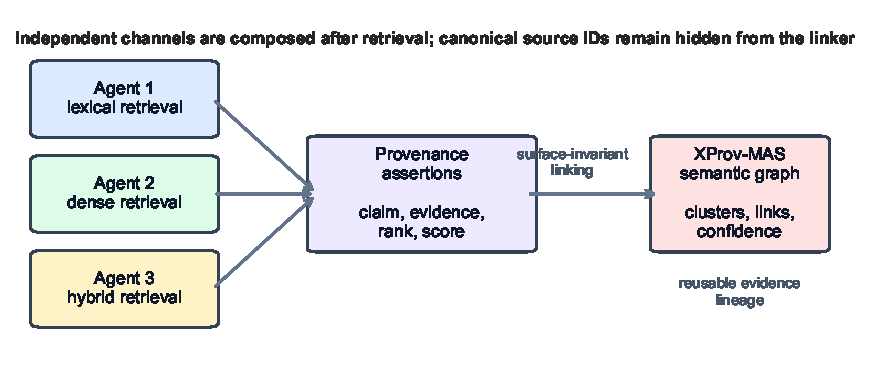
\includegraphics[width=0.92\textwidth]{framework}
\caption{XProv-MAS architecture. Independent retrieval channels emit provenance assertions; the graph links report surfaces while canonical source identifiers remain hidden from the linker and are used only for evaluation.}
\label{fig:framework}
\end{figure}

\subsection{Data, Agents, and Baselines}

The primary campaign uses all 19,998 FEVER development claims and the official June 2017 Wikipedia snapshot; 300 SciFact development claims and the complete 5,183-abstract corpus; and 1,221 PUBHEALTH development claims with an open article collection. A secondary PUBHEALTH audit covers the 33 development claims with at least one of 4,200 official evidence documents. PAWS train, validation, and test pairs provide an external semantic audit. The resulting primary runs emit 299,970 FEVER, 4,500 SciFact, 18,315 PUBHEALTH, and 495 evidence-document assertions.

Three deterministic channels rank the same candidate corpus: a lexical TF--IDF agent, a dense MiniLM agent, and a hybrid agent combining normalized lexical and dense scores with weights $0.35$ and $0.65$. Each emits its top five candidates. Lexical assertions retain title-plus-text surfaces; dense assertions remove the title and apply a reproducible transformation that replaces at most eight words from a fixed synonym inventory; hybrid assertions use a compact title-plus-text surface. The transformation changes wording but not the ranked candidate or hidden source.

The isolated baseline creates no edges. The lexical and dense baselines apply $J\geq0.42$ and $D\geq0.70$, respectively. All thresholds are fixed across primary datasets. Gold source identifiers are stored in raw assertion records and are consulted only after ranking and graph construction; they are never features of a linker.

\subsection{Metrics and Experimental Protocol}

For each assertion pair, hidden-source equality defines the gold relation. We report pair precision, recall, and F1 over all pairs in a record. Cross-agent rephrase match is the fraction of cross-channel, same-source pairs that fall in one component. Source precision, recall, and F1 measure the upstream retrieval ceiling; these values are shared by linkers using the same top-five lists. Composable-source rate is the fraction of retrieved gold sources with reports from at least two channels that collapse to one component. It differs from pairwise F1 because a component can preserve a source while also absorbing unrelated assertions.

We use 2,000-resample record-level bootstrap intervals and paired differences. The record, rather than the assertion pair, is the resampling unit because pairs within a claim are correlated. The primary runner is deterministic for a fixed model and manifest. The SciFact top-$k$ audit uses $k\in\{1,3,5,10\}$, and a separate threshold grid reports sensitivity without replacing the predeclared primary setting. All raw assertions, per-record metrics, summaries, bootstrap outputs, and figures are generated artifacts, allowing manuscript values to be traced to executed files.

\begin{table}[t]
\centering
\caption{Primary datasets and fixed experimental scale.}
\label{tab:data}
\scriptsize
\setlength{\tabcolsep}{1.5pt}
\begin{tabular}{lrrr}
\toprule
Dataset & Records & Cand. & Asserts.\\
\midrule
FEVER dev. & 19,998 & 2,860 & 299,970\\
SciFact dev. & 300 & 5,183 & 4,500\\
PUBHEALTH dev. & 1,221 & 11,053 & 18,315\\
PUBHEALTH ev. & 33 & 4,200 & 495\\
\bottomrule
\end{tabular}
\end{table}

\section{Results}

\subsection{Primary Composition Results}

Table~\ref{tab:primary} shows the fixed-configuration results. Lexical linking is a strong baseline on these controlled assertion surfaces. XProv-MAS is not a universal pairwise-accuracy improvement: its semantic gate trades precision for rephrase-aware composition. Its intended benefit is clearest in the composable-source column, which records whether a source reported by multiple channels becomes one reusable component.

\begin{table}[t]
\centering
\caption{Primary provenance-composition results. Values are means over query records; source F1 is the upstream retrieval ceiling.}
\label{tab:primary}
\small
\resizebox{\textwidth}{!}{%
\begin{tabular}{llrrrrr}
\toprule
Dataset & Linker & Pair P & Pair R & Pair F1 & Rephrase & Composable\\
\midrule
FEVER & Lexical & \FEVERLexicalPrecision & \FEVERLexicalRecall & \FEVERLexicalFOne & 1.000 & \FEVERLexicalComposable\\
 & Dense & \FEVERDensePrecision & \FEVERDenseRecall & \FEVERDenseFOne & 1.000 & \FEVERDenseComposable\\
 & XProv-MAS & \FEVERXProvPrecision & \FEVERXProvRecall & \FEVERXProvFOne & 1.000 & \FEVERXProvComposable\\
\midrule
SciFact & Lexical & \SciFactLexicalPrecision & \SciFactLexicalRecall & \SciFactLexicalFOne & 1.000 & \SciFactLexicalComposable\\
 & Dense & \SciFactDensePrecision & \SciFactDenseRecall & \SciFactDenseFOne & 1.000 & \SciFactDenseComposable\\
 & XProv-MAS & \SciFactXProvPrecision & \SciFactXProvRecall & \SciFactXProvFOne & 1.000 & \SciFactXProvComposable\\
\midrule
PUBHEALTH & Lexical & \PubHealthLexicalPrecision & \PubHealthLexicalRecall & \PubHealthLexicalFOne & \PubHealthLexicalRephrase & \PubHealthLexicalComposable\\
 & Dense & \PubHealthDensePrecision & \PubHealthDenseRecall & \PubHealthDenseFOne & 1.000 & \PubHealthDenseComposable\\
 & XProv-MAS & \PubHealthXProvPrecision & \PubHealthXProvRecall & \PubHealthXProvFOne & 1.000 & \PubHealthXProvComposable\\
\midrule
Evidence subset & Lexical & \PubHealthEvidenceLexicalPrecision & \PubHealthEvidenceLexicalRecall & \PubHealthEvidenceLexicalFOne & \PubHealthEvidenceLexicalRephrase & \PubHealthEvidenceLexicalComposable\\
 & XProv-MAS & \PubHealthEvidenceXProvPrecision & \PubHealthEvidenceXProvRecall & \PubHealthEvidenceXProvFOne & 1.000 & \PubHealthEvidenceXProvComposable\\
\bottomrule
\end{tabular}}
\end{table}

On FEVER, XProv-MAS reaches pairwise F1 \FEVERXProvFOne{} versus \FEVERLexicalFOne{} for lexical linking. The high scores reflect short, page-level evidence surfaces with distinctive words; they are a scale test rather than evidence that lexical matching is semantically sufficient in general. The run processes all 19,998 claims and preserves an assertion-level graph at 299,970 rows.

SciFact exposes a stronger retrieval boundary. XProv-MAS reaches \SciFactXProvFOne{} versus \SciFactLexicalFOne{}, while the source-F1 ceiling is only \SciFactXProvSourceFOne{}. A graph cannot recover an abstract that no channel retrieved. Thus source retrieval and provenance composition are separate failure classes: the former limits the available evidence entities, while the latter determines how those entities are composed.

PUBHEALTH provides the clearest operational tradeoff. XProv-MAS lowers pairwise F1 from the lexical value \PubHealthLexicalFOne{} to \PubHealthXProvFOne{}, but increases composable-source rate from \PubHealthLexicalComposable{} to \PubHealthXProvComposable{}. It retains a 1.000 rephrase match. On the official evidence-document subset, XProv-MAS reaches F1 \PubHealthEvidenceXProvFOne{} and composability \PubHealthEvidenceXProvComposable{}, compared with \PubHealthEvidenceLexicalFOne{} and \PubHealthEvidenceLexicalComposable{} for lexical linking. This is the intended use case: composing transformed reports while retaining an auditable tradeoff.

\begin{figure}[t]
\centering
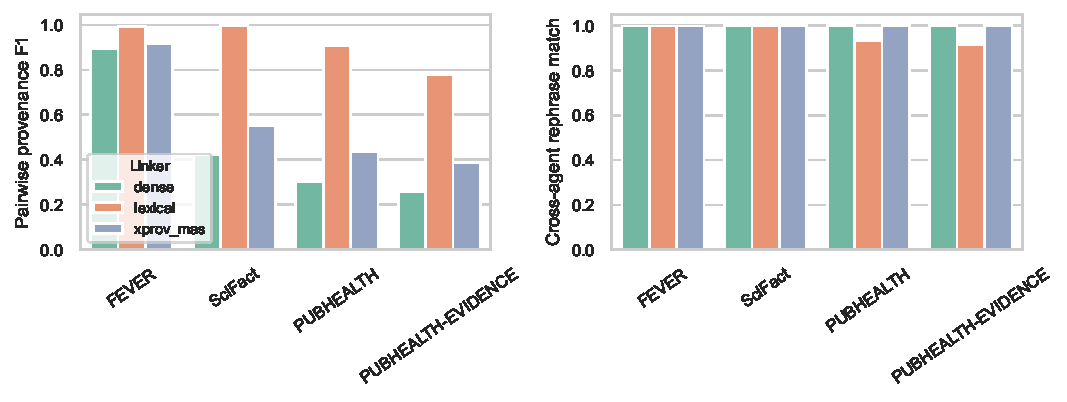
\includegraphics[width=\columnwidth]{performance}
\caption{Primary pairwise provenance F1 and cross-agent rephrase match. XProv-MAS preserves transformed-source composition but does not uniformly improve pairwise precision.}
\label{fig:performance}
\end{figure}

\subsection{Retrieval Depth, Uncertainty, and Boundaries}

The top-five constraint is consequential. In the executed SciFact audit, XProv-MAS pairwise F1 is 0.823 at $k=1$, 0.672 at $k=3$, \SciFactXProvFOne{} at $k=5$, and 0.419 at $k=10$; source F1 is 0.379, 0.198, \SciFactXProvSourceFOne{}, and 0.072, respectively. Rephrase match rises from 0.887 at $k=1$ to 1.000 at deeper settings, while composability increases. Deeper retrieval exposes more reports to the graph, increasing opportunities for composition and false links simultaneously.

The source-F1 ceiling is shared by all linkers because candidate lists are fixed. It is approximately \FEVERXProvSourceFOne{} on FEVER, \SciFactXProvSourceFOne{} on SciFact, and \PubHealthXProvSourceFOne{} on PUBHEALTH. The evidence subset has source F1 0.205. These numbers make clear that XProv-MAS evaluates composition conditional on retrieval; an end-to-end evidence system must report both layers.

Record-level bootstrap intervals confirm the precision tradeoff. XProv-MAS pairwise F1 is \FEVERXProvFOneCI{} on FEVER, \SciFactXProvFOneCI{} on SciFact, \PubHealthXProvFOneCI{} on PUBHEALTH, and \PubHealthEvidenceXProvFOneCI{} on the evidence subset. The paired differences from lexical linking are \FEVERXProvPairFOneDelta{}, \SciFactXProvPairFOneDelta{}, \PubHealthXProvPairFOneDelta{}, and \PubHealthEvidenceXProvPairFOneDelta{}. Conversely, the composability differences are \PubHealthXProvComposableDelta{} and \PubHealthEvidenceXProvComposableDelta{} on the two PUBHEALTH evaluations.

\begin{table}[t]
\centering
\caption{SciFact depth audit for XProv-MAS.}
\label{tab:topk}
\small
\begin{tabular}{rrrr}
\toprule
$k$ & Pair F1 & Rephrase & Source F1\\
\midrule
1 & 0.823 & 0.887 & 0.379\\
3 & 0.672 & 1.000 & 0.198\\
5 & \SciFactXProvFOne & 1.000 & \SciFactXProvSourceFOne\\
10 & 0.419 & 1.000 & 0.072\\
\bottomrule
\end{tabular}
\end{table}

\begin{table}[t]
\centering
\caption{Record-level 95\% bootstrap intervals for XProv-MAS pairwise F1.}
\label{tab:uncertainty}
\small
\begin{tabular}{lr}
\toprule
Dataset & XProv-MAS 95\% CI\\
\midrule
FEVER & \FEVERXProvFOneCI\\
SciFact & \SciFactXProvFOneCI\\
PUBHEALTH & \PubHealthXProvFOneCI\\
Evidence & \PubHealthEvidenceXProvFOneCI\\
\bottomrule
\end{tabular}
\end{table}

The two audit tables make the operating tradeoff explicit. Shallow retrieval can be relatively source-pure but misses evidence; deeper retrieval increases the number of candidate reports and therefore the opportunity for both correct composition and false bridging. The intervals are record-level rather than pair-level, so they reflect variation across claims instead of treating the many pairs emitted by one claim as independent observations.

\begin{table}[t]
\centering
\caption{Upstream retrieval ceiling shared by graph strategies.}
\label{tab:retrieval}
\small
\begin{tabular}{lrrr}
\toprule
Dataset & Precision & Recall & F1\\
\midrule
FEVER & 0.088 & 0.977 & \FEVERXProvSourceFOne\\
SciFact & 0.076 & 0.961 & \SciFactXProvSourceFOne\\
PUBHEALTH & 0.102 & 0.896 & \PubHealthXProvSourceFOne\\
Evidence & 0.241 & 0.268 & 0.205\\
\bottomrule
\end{tabular}
\end{table}

\subsection{Robustness and Threshold Sensitivity}

The PAWS audit tests the semantic primitives outside the graph. Lexical AUC is approximately 0.50 on all official splits, while dense MiniLM similarity reaches \PAWSTrainDenseAUC, \PAWSValidationDenseAUC, and \PAWSTestDenseAUC. The fixed hybrid scorer reaches only \PAWSTrainHybridAUC, \PAWSValidationHybridAUC, and \PAWSTestHybridAUC. Dense similarity is therefore more informative than lexical overlap for difficult paraphrases, but the hybrid combination is not automatically better. The 1.000 rephrase-match values in the main campaign should be interpreted as invariance to the specified conservative transformation, not as general paraphrase competence.

\begin{figure}[t]
\centering
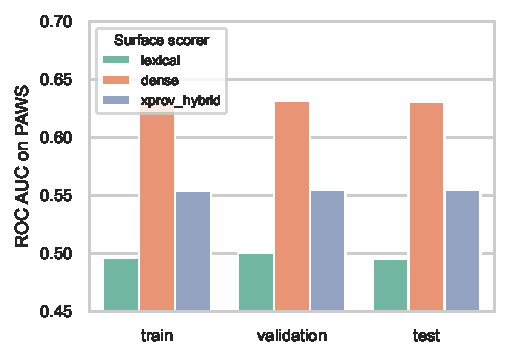
\includegraphics[width=\columnwidth]{paws_robustness}
\caption{PAWS audit. Dense similarity is consistently more informative than lexical overlap, while the fixed hybrid combination is not superior to the dense channel.}
\label{fig:paws}
\end{figure}

The SciFact threshold grid gives primary pairwise F1 \SciFactSensitivityPrimary{} and reaches \SciFactSensitivityBest{} at a stricter observed operating point. The training-split audit reaches \SciFactTrainBest{}, but this value is not substituted into the cross-domain primary table. The surface is not monotonic because union--find components change discontinuously when a bridge edge is added or removed. Thresholds are therefore scientific parameters that should be calibrated on a validation domain and logged as parameter provenance.

\begin{figure}[t]
\centering
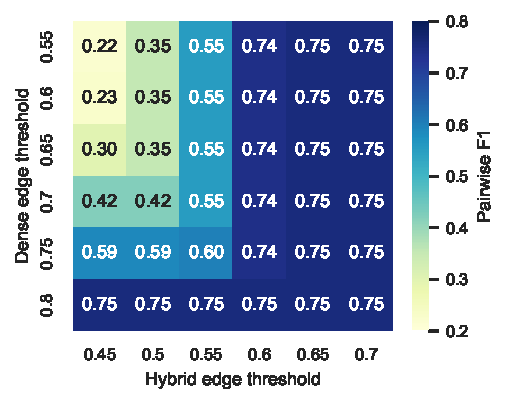
\includegraphics[width=\columnwidth]{threshold_sensitivity}
\caption{SciFact threshold sensitivity. The primary setting is $(\tau_D,\tau_H)=(0.60,0.55)$; graph behavior changes materially across the grid.}
\label{fig:sensitivity}
\end{figure}

\subsection{Failure Analysis and Responsible Use}

The most important failure is a false merge: two topical but distinct sources can become one component when moderate lexical and dense similarities combine through transitive closure. A second failure is a missed edge when a rephrase removes domain-specific terms or when a candidate surface is too long for a compact representation. A third failure is upstream; when no channel retrieves a gold source, graph composition cannot recover it. Multi-source claims are harder because a component must preserve branch distinctions, not merely connect same-source reports.

Mean scores hide long tails. XProv-MAS has median pairwise F1 of 1.000 on FEVER, 0.500 on SciFact, and 0.327 on PUBHEALTH, with 10th percentiles of 0.667, 0.215, and 0.143. The evidence-document subset has median 0.294 and a small-sample interval. No claim-level veracity predictor is trained here; differences by label or domain should not be interpreted as factuality performance.

Same-source equality is a useful provenance construct but is not semantic equivalence or entailment. A graph can link multiple reports of a source that does not support the claim, and it can separate different sources that provide equivalent evidence. Similarly, the controlled transformation is not a generative paraphrase distribution, and the benchmark candidate collections are not an Internet-scale index. These limitations are addressed by separating source retrieval from linking, including PAWS, reporting bootstrap uncertainty, and keeping hidden identifiers out of the linker.

For responsible deployment, a user interface should distinguish source identity, semantic compatibility, entailment, and veracity; show retrieval rank and transformation history; preserve unresolved branches; and avoid presenting several reports of one source as independent corroboration. High-stakes use should add span-level evidence, contradiction edges, versioned source locators, and human review. The current assertion schema provides a place for these additions without changing the basic graph interface.

\section{Discussion and Conclusion}

XProv-MAS answers the study questions with a qualified result. The graph creates measurable composition beyond isolation and preserves same-source cross-agent links under the implemented rephrasing. The same schema transfers across general encyclopedic evidence, scientific abstracts, public-health articles, and harvested evidence documents. However, lexical linking remains more precise on the controlled surfaces, PAWS shows that dense similarity alone does not solve hard paraphrases, and source retrieval remains an upstream bottleneck.

The appropriate interpretation is architectural. XProv-MAS is an intermediate provenance-composition layer, not a retriever, fact verifier, or calibrated uncertainty model. Agents should emit stable assertion objects containing claim and evidence spans, retrieval scores, source locators, transformation history, and model versions. A verifier can then attach canonical evidence or contradiction relations without discarding the original reports. This separation allows retrieval and linking to be improved independently and makes false merges visible rather than silently flattening them into prose.

Future work should evaluate independently sampled generative paraphrases, multilingual and longer-form evidence, held-out threshold calibration, entailment-aware edges, contradiction relations, and human review time. It should also test genuinely independent retrieval trajectories rather than only lexical, dense, and hybrid views of one candidate corpus. The present study establishes a reproducible baseline: it measures source-oblivious composition at scale, demonstrates the intended rephrase behavior on real benchmark evidence, reports an operational composability gain on PUBHEALTH, and records where the layer fails.


\begin{multicols}{2}
\bibliographystyle{spmpsci}
\bibliography{references}
\end{multicols}

\end{document}
